\documentclass{article}
\usepackage{amsmath,amssymb}
\usepackage{fullpage}
\usepackage{mathrsfs}
\usepackage{setspace}
\usepackage{graphicx}
\usepackage{caption,subcaption}
\usepackage{listings}
\renewcommand{\baselinestretch}{1.4}
\pagestyle{empty}
\usepackage{color}
\definecolor{dkgreen}{rgb}{0,0.6,0}
\definecolor{gray}{rgb}{0.5,0.5,0.5}
\definecolor{mauve}{rgb}{0.58,0,0.82}

\lstset{frame=tb,
	language=Matlab,
	aboveskip=3mm,
	belowskip=3mm,
	showstringspaces=false,
	columns=flexible,
	basicstyle={\small\ttfamily},
	numbers=none,
	numberstyle=\tiny\color{gray},
	keywordstyle=\color{blue},
	commentstyle=\color{dkgreen},
	stringstyle=\color{mauve},
	breaklines=true,
	breakatwhitespace=true,
	tabsize=4
}

\usepackage[]{algorithm2e}
%\usepackage{algorithm}

\title{Implementation of Jacobi and Gauss-Seidel Method} 
\author{Jingmin Sun}
\date{\today}
\begin{document}
\maketitle
\tableofcontents
\pagebreak

\section{Overview}
In this project, I implement two algorithms (Jacobi and Gauss-Seidel) on simple and random linear system. In both algorithm, I set the stopping criteria to be the small tolerance of relative error, and the maximum number of iteration.

\section{Algorithm}
\hrule
Algorithm (Jacobi Method):
\hrule
\begin{algorithm}[H]
\SetAlgoLined
Initialization: $A \succ 0$, diagonally dominant, $tol>0,\; b, \; x^0, \; imax, \; error = \infty $ and $x_r$, such that $Ax_r=b$.\\
\For{k=0,1,2,$\cdots imax$}{\eIf{$error\leq tol$}{stop}{
   $ \delta = \sum_{j=1}^n A_{ij}\cdot x_j^k - A_{ii}\cdot x_i^k= A_{i,:}\cdot x^k- A_{ii}\cdot x_i^k$\\
    $x_{i}^{k+1}=\dfrac{b_i-\delta}{A_{ii}}$\\
}$error =\dfrac{||x^{k+1} -x_r||}{||x_{k+1}||}$}
\end{algorithm}

~\\

\hrule
Algorithm (Gauss-Seidel Method):
\hrule
\begin{algorithm}[H]
\SetAlgoLined
Initialization: $A \succ 0$, diagonally dominant, $tol>0,\; b, \; x^0,  \; imax, \; error = \infty $ and $x_r$, such that $Ax_r=b$.\\
\For{k=0,1,2,$\cdots imax$}{\eIf{$error\leq tol$}{stop}{
   $ \delta = \sum_{j=1}^{i-1} A_{ij}\cdot x_j^{k+1} +\sum_{j=i+1}^{n} A_{ij}\cdot x_j^k $\\
    $x_{i}^{k+1}=\dfrac{b_i-\delta}{A_{ii}}$
}$error =\dfrac{||x^{k+1} -x_r||}{||x_{k+1}||}$}
\end{algorithm}

\section{Implementation of Methods}
\subsection{Jacobi Method}
\lstinputlisting[language=Matlab,caption={Jacobi Method},frame=single,numbers=left, stepnumber=1, firstline=1]{Jacobi.m}
\subsection{Gauss-Seidel Method}
\lstinputlisting[language=Matlab,caption={Gauss-Seidel method},frame=single, numbers=left, stepnumber=1, firstline=1]{GaussSeidel.m}

\section{Test of the algorithm}
\subsection{Simple case}
\subsubsection{Code}
\lstinputlisting[language=Matlab,caption={Simple case},frame=single, numbers=left, stepnumber=1, firstline=1]{Jaco_GS_test.m}

\subsubsection{Result}
The result is attached in the back of the report, and the graph is:

\begin{figure}[ht]
\centering
  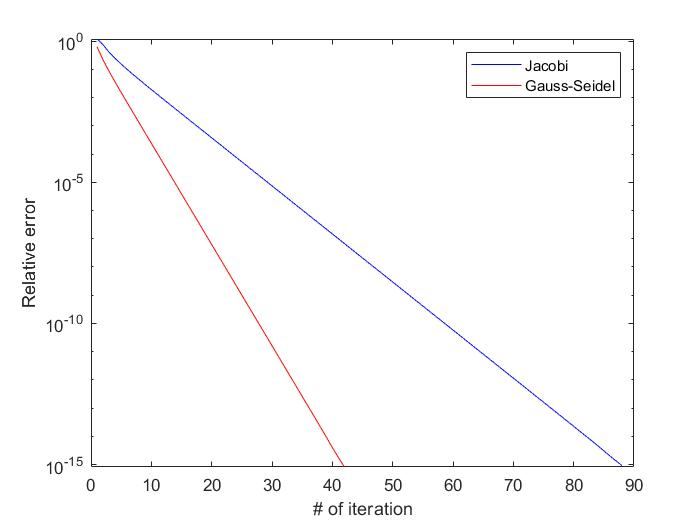
\includegraphics[width = 6cm]{simplecase.jpg}
  \caption {Simple case}
  \end{figure}

 \subsubsection{Observation}
 We can easily see that the Jacobi method is much slower than the Gauss-Seidel method, and it is because that Gauss-Seidel uses the latest updated version of the $x_j$, so we do not waste our effort on working with the old information.
  
\subsection{Random case}
\subsubsection{The derivation of diagonally dominant matrix}

The diagonal dominant matrix are generated simply by replacing the absolute value of diagonal entries by the sum of the absolute value of each entry in the row and a bit more.

\subsubsection{Code}
\lstinputlisting[language=Matlab,caption={Random case}, numbers=left, stepnumber=1, firstline=1,frame=single]{Jaco_GS_test_rand.m}

\subsubsection{Result}
The result is attached in the back of the report, and the graph is:

\begin{figure}[ht]
\centering
\caption {Random 100 x 100 case}
  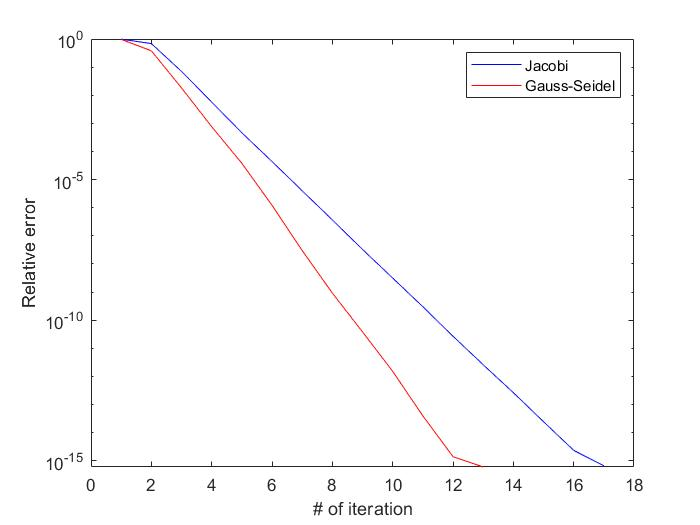
\includegraphics[width=6cm]{randomcase.jpg}
  \end{figure} 
  \subsubsection{Observation}
  
We can get the similar result as before, but we can see that the difference between two method are relatively smaller than before, and the total number of iterations for both methods are small as well.

\section{Development}
As the claim I made before, I change the size of the matrix to different scale and gives me the following result:
  \begin{figure}[ht]
  \centering
  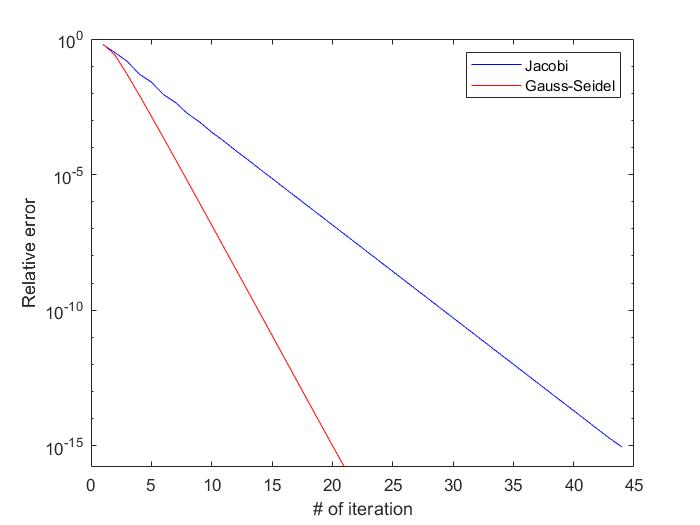
\includegraphics[width=6cm]{randomcase44.jpg}
  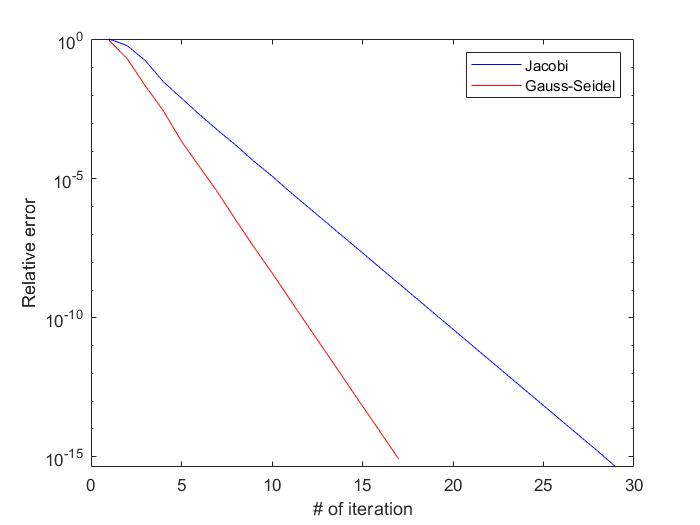
\includegraphics[width=6cm]{randomcase1010.jpg}
  \caption{Random 4 x 4 on the left and 10 x 10 on the right}
  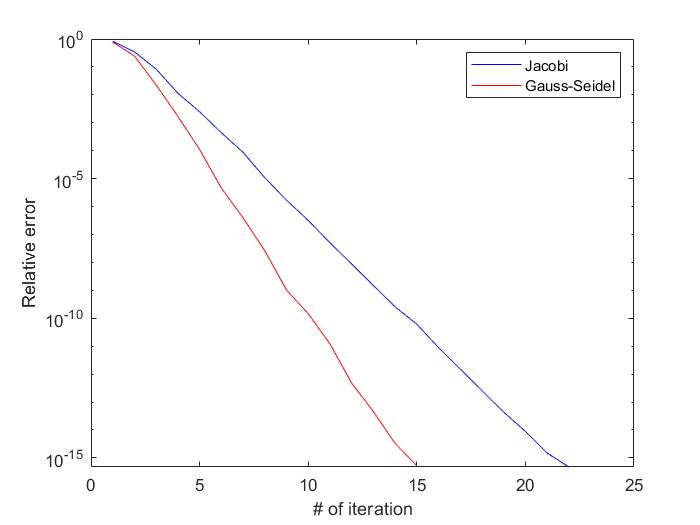
\includegraphics[width=6cm]{randomcase2020.jpg}
  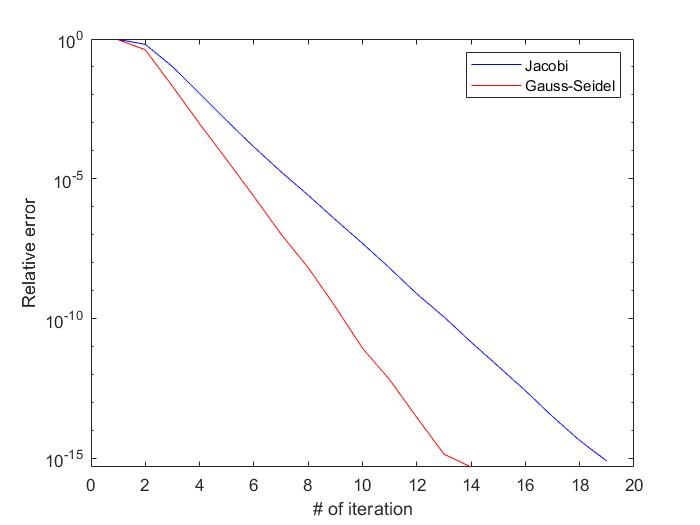
\includegraphics[width=6cm]{randomcase5050.jpg}
  \caption{Random 20 x 20 on the left and 50 x 50 on the right}
   \end{figure}
   
   And we can observe that as the size of the matrix increases, the number of iterations of both method are decreased, and the difference of two methods is decreasing as well.
   
   And this phenomenon can be explained:   
   Since for the Jacobi method $B = D^{-1}(U+L)$, and for Gauss-Seidel method $B = (D+L)^{-1}U$,  $\tilde{b} = D^{-1}b$, and the diagonal matrix is strictly dominant, with the knowledge of when $r$ (size of the matrix) goes up, each element in a row plays a smaller and smaller role in the sum of that row, and the diagonal entries are completely dominant compared to other entries in matrix $A$, so that each entry in both $B$ will be relative small, and $x$ can be decrease sufficiently in each iteration, so that the number of iteration will be decrease. And at the same time, the difference between two $B$s will decrease as well, and the difference between two methods will decrease.

We can check for that by checking the spectrum radius of B with the code
\lstinputlisting[language=Matlab,caption={Spectral radius},frame=single,numbers=left, stepnumber=1, firstline=1]{spec_rad_B.m}

and with the result that \lstinputlisting[language=Matlab,caption={Output}]{sr_B.txt}

Since we know that the one with larger spectral radius in absolute value would have slower convergence rate, and that the convergence of x is closed related with the matrix B, the result above enhanced my statement above that GS method is always faster than Jacobi method, and with the increase of the size of the matrix, the algorithm converges faster.
\section{Appendix}
\lstinputlisting[language=Matlab,caption={Simple output}]{simpleout.txt}
\lstinputlisting[language=Matlab,caption={Random output}]{randomout.txt}
\end{document}